% ****** Start of file apssamp.tex ******
%
%   This file is part of the APS files in the REVTeX 4.1 distribution.
%   Version 4.1r of REVTeX, August 2010
%
%   Copyright (c) 2009, 2010 The American Physical Society.
%
%   See the REVTeX 4 README file for restrictions and more information.
%
% TeX'ing this file requires that you have AMS-LaTeX 2.0 installed
% as well as the rest of the prerequisites for REVTeX 4.1
%
% See the REVTeX 4 README file
% It also requires running BibTeX. The commands are as follows:
%
%  1)  latex apssamp.tex
%  2)  bibtex apssamp
%  3)  latex apssamp.tex
%  4)  latex apssamp.tex
%
\documentclass[
reprint,
superscriptaddress,
% groupedaddress,
amsmath,
amssymb,
aps,
prd
% prl,
% showpacs,
%unsortedaddress,
%runinaddress,
%frontmatterverbose, 
%preprint,
%showpacs,preprintnumbers,
%nofootinbib,
%nobibnotes,
%bibnotes,
%pra,
%prb,
%rmp,
%prstab,
%prstper,
%floatfix,
]{revtex4-1}

\usepackage{graphicx}% Include figure files
\usepackage{dcolumn}% Align table columns on decimal point
\usepackage{bm}% bold math
\usepackage{amssymb}   % for math
\usepackage{hyperref}% add hypertext capabilities
\usepackage{aas_macros}
\usepackage[caption=false]{subfig}
%\usepackage[mathlines]{lineno}% Enable numbering of text and display math
%\linenumbers\relax % Commence numbering lines

%\usepackage[showframe,%Uncomment any one of the following lines to test 
%%scale=0.7, marginratio={1:1, 2:3}, ignoreall,% default settings
%%text={7in,10in},centering,
%%margin=1.5in,
%%total={6.5in,8.75in}, top=1.2in, left=0.9in, includefoot,
%%height=10in,a5paper,hmargin={3cm,0.8in},
%]{geometry}

\newcommand{\HI}{H\,{\sc i}}

\begin{document}

\preprint{APS/123-QED}

\title{Detecting Cosmic Reionization using Bi-Spectrum Phase}% Force line breaks with \\
% \thanks{A footnote to the article title}%

\author{Nithyanandan Thyagarajan}
\email{t\_nithyanandan@nrao.edu}
\homepage{https://tnithyanandan.wordpress.com/}
\thanks{Nithyanandan Thyagarajan is a Jansky Fellow of the National Radio Astronomy Observatory.}
\affiliation{National Radio Astronomy Observatory, Socorro, NM 87801, USA}
\affiliation{Arizona State University, School of Earth and Space Exploration, Tempe, AZ 85287, USA}
% \altaffiliation[Also at ]{Physics Department, XYZ University.}%Lines break automatically or can be forced with \\
\author{Chris L. Carilli}%
% \email{Second.Author@institution.edu}
\affiliation{National Radio Astronomy Observatory, Socorro, NM 87801, USA}
\affiliation{Astrophysics Group, Cavendish Laboratory, University of Cambridge, Cambridge CB3 0HE, UK}

% \collaboration{MUSO Collaboration}%\noaffiliation

\author{Bojan Nikolic}
% \homepage{http://www.Second.institution.edu/~Charlie.Author}
\affiliation{Astrophysics Group, Cavendish Laboratory, University of Cambridge, Cambridge CB3 0HE, UK}%
% \affiliation{
%  Third institution, the second for Charlie Author
% }%

% \collaboration{CLEO Collaboration}%\noaffiliation

\date{\today}% It is always \today, today,
             %  but any date may be explicitly specified

\begin{abstract} 
  Detecting neutral Hydrogen (\HI) via the 21~cm line emission from
  the intergalactic medium at $z\gtrsim 6$ has been identified as one
  of the most promising probes of the epoch of cosmic reionization --
  a major phase transition of the Universe. However, these studies face the severe challenge imposed
  by the bright foreground emission from cosmic objects: current
  techniques require precise instrumental calibration to separate
  the weak \HI\ line signal from the foreground continuum emission. We
  propose to mitigate this calibration requirement by using the phase
  of the bi-spectrum from interferometric measurements. Bi-spectrum
  phase is unaffected by antenna-based direction-independent calibration
  errors and hence for a compact array it depends on the sky brightness
  distribution only (subject to the usual thermal-like noise).
  We show that the bi-spectrum phase of foreground synchrotron continuum has
  a characteristically smooth spectrum relative to the cosmological line
  signal. The two can be separated effectively by exploiting this
  spectral difference using Fourier techniques, while
  eliminating the need for precise antenna-based calibration of
  phases introduced by the instrument, and the ionosphere, inherent in
  existing approaches. Using fiducial models for continuum
  foregrounds, and for the cosmological \HI\ signal, we show the
  latter should be detectable in bi-spectrum phase spectra, with
  reasonable significance at
  $|k_\parallel| \gtrsim 0.5\,h$~Mpc$^{-1}$, using existing
  instruments.
\end{abstract}

% \begin{abstract}
% An article usually includes an abstract, a concise summary of the work
% covered at length in the main body of the article. 
% \begin{description}
% \item[Usage]
% Secondary publications and information retrieval purposes.
% \item[PACS numbers]
% May be entered using the \verb+\pacs{#1}+ command.
% \item[Structure]
% You may use the \texttt{description} environment to structure your abstract;
% use the optional argument of the \verb+\item+ command to give the category of each item. 
% \end{description}
% \end{abstract}

\pacs{}% PACS, the Physics and Astronomy
                             % Classification Scheme.
%\keywords{Suggested keywords}%Use showkeys class option if keyword
                              %display desired

% \pacs{Valid PACS appear here}% PACS, the Physics and Astronomy
%                              % Classification Scheme.
% %\keywords{Suggested keywords}%Use showkeys class option if keyword
%                               %display desired

\maketitle

%\tableofcontents

\section{Introduction}\label{sec:intro}

The hydrogen gas that dominates the baryon content of the Universe has undergone two phase transitions over cosmic history. The first was the transition from fully ionized to fully neutral gas during cosmic \emph{recombination\/} $\sim 300,000$ years after the Big Bang ($z\approx 1100$). This epoch has been quantified in exquisite detail through cosmic microwave background radiation studies \cite{planck15i}. The second transition is known as cosmic \emph{reionization}, when light from the first stars and black holes reionized the neutral Hydrogen (\HI) gas that pervaded the early Universe. Current indirect constraints suggest this second transition occurred a few hundred Myr to $\sim 1$~Gyr ($z\gtrsim 6$) \cite{gre17a} after the Big Bang. During this epoch, the photon-to-baryon ratio eventually exceeded unity, reionizing the entire Universe except gas bound to galaxies. The astrophysical processes during this epoch shaped the evolution of galaxies and large-scale structure. However, unlike recombination, the timing and process of cosmic reionization remain poorly understood. The redshifted 21~cm spectral line from the electron spin-flip transition in \HI\ atom, has been recognized as the most promising tool to unravel the physical processes involved in cosmic reionization, and the evolution of large scale structure during the formation of the first galaxies \cite{sun72,sco90,mad97,toz00,ili02,fan02,fan06,bar07,mor10}.

Our Galaxy and intervening radio galaxies emit synchrotron radiation in the same frequency band ($\sim$~100--200~MHz) as the redshifted \HI\ signal from the epoch of reionization (EoR), with a brightness temperature roughly $\gtrsim 10^4$ times higher than the EoR \HI\ signal. However, the synchrotron foregrounds have a smooth spectrum whereas the EoR \HI\ signal will appear as small fluctuations superimposed on the smooth foreground spectrum. The hope of separating the cosmic line signal from the Galactic and extragalactic foregrounds has spawned a number of low-frequency instruments (eg. \cite{par10,tin13,van13}), with sensitivities sufficient for a statistical detection of the EoR \HI\ signal using power spectrum methodology \cite{thy13,bea13}.  However, despite obtaining sufficient observational data, these experiments remain dynamic range limited due to the coupling of the strong foreground emission to the EoR \HI\ signal via instrumental effects, particularly systematics related to precision of calibration, and the intrinsic chromatic instrumental response \cite{thy15a,thy15b,thy16,dat09,dat10,tro16, pac13,ali15,patil17,pob15,liu10,zhe14,barry16,sie17,dil17}. 

We present an alternate approach using the phase of the complex bi-spectrum (also referred to in radio interferometry as closure phase) to detect the signal from the EoR. This quantity is impervious to antenna-based complex gains introduced by the instrument and the ionosphere, and thus can remove the need for high-precision calibration currently impeding existing approaches\cite{car16}.

\section{Properties of Bi-spectrum Phase}\label{sec:CPinfo}

The bi-spectrum in the context of interferometry has been investigated in \cite{jen58,kul89,tay99,tho01,mon06} and recently revisited in \cite{car18}. Consider a triad of antennas $a$, $b$, and $c$ indexed by $i\in \{a, b, c\}$, and antenna pairs indexed by $ij\in \{ab, bc, ca\}$. Bi-spectrum is defined as:
\begin{align}
  B_\nabla(f) &= \prod_{ij} V_{ij}(f),
\end{align}
where, $V_{ij}(f)$ denotes spatial coherence spectrum measured between antenna pair $ij$ at frequency $f$. The instrument and/or ionosphere may introduce complex antenna-based gains, $g_i$. Then, 
\begin{align}\label{eqn:vis-antgains}
  V_{ij}^\textrm{m}(f) &= g_i(f)\, g_j^*(f)\, V_{ij}^\textrm{T}(f) + V_{ij}^\textrm{N}(f),
\end{align}
where, the measured spatial coherence, $V_{ij}^\textrm{m}(f)$, is the sum of contributions from thermal-like noise, $V_{ij}^\textrm{N}(f)$, and true spatial coherence, $V_{ij}^\textrm{T}(f)$ of the sky, corrupted by the antenna gains. Then the measured bi-spectrum is:
\begin{align}\label{eqn:bispectrum-terms}
  B_\nabla^\textrm{m} &= B_\nabla^\textrm{T}\prod_i |g_i|^2 \,\, + \,\, \textrm{noise-like terms}
\end{align}
where, the dependence on $f$ has been omitted for convenience hereafter unless indicated otherwise.
All noise-like terms on the R.H.S. are uncorrelated and have zero mean due to the presence of $V_{ij}^\textrm{N}$. Hence, $\langle B_\nabla^\textrm{m}\rangle = \langle B_\nabla^\textrm{T} \prod_i |g_i|^2 \rangle$.

Denoting the bi-spectrum phase\footnote{Note that this usage of bi-spectrum phase, $\phi_\nabla^\textrm{m}$, differs from cosmologists' use of bi-spectrum, $B_\nabla^\textrm{m}$. The latter is usually averaged spherically in $k$-bins and still requires precise antenna calibration, whereas we use the power spectrum of $e^{i\phi_\nabla^\textrm{m}}$ and is not subject to the high-precision calibration requirement.} as $\phi_\nabla$, 
\begin{align}
  \phi_\nabla^\textrm{m} &= \sum_{ij}\phi_{ij}^\textrm{m} = \phi_\nabla^\textrm{T} + \delta\phi_\nabla^\textrm{N} \label{eqn:cpphase-sum},
\end{align}
where, $\delta\phi_\nabla^\textrm{N}$ is the perturbation due to thermal noise superimposed on true phase, $\phi_\nabla^\textrm{T}$. $\phi_{ij}^\textrm{m} = \phi_i - \phi_j + \phi_{ij}^\textrm{T} + \delta\phi_{ij}^\textrm{N}$, and $\phi_i$ denote the phases of the measured spatial coherence, $V_{ij}^\textrm{m}$, and the complex antenna gain $g_i$, respectively. The measured bi-spectrum phase, $\phi_\nabla^\textrm{m}$, is independent of the antenna gains and identical to that of the true bi-spectrum corrupted only by noise. Hence, $\phi_\nabla^\textrm{m}$ contains information purely about the sky's spatial structure, and has the properties \cite{mon07}: translation invariance to sky structure; $\phi_\nabla^\textrm{T}=0$ or $\pi$ implies centrosymmetric structure, while other values imply a skewed structure; and, a resolved structure is required for $\phi_\nabla^\textrm{T}\ne 0$.

Defining the signal-to-noise ratio in the spatial coherence as $\rho_{ij}^\textrm{N} = |V_{ij}^\textrm{T}|/|V_{ij}^\textrm{N}|$, where, $V_{ij}^\textrm{N}$ includes both real and imaginary parts, the probability distribution of $\delta\phi_{ij}^\textrm{N}$ depends on $\rho_{ij}^\textrm{N}$ as \cite{cra89}:
\begin{align}
  P(\delta\phi_{ij}^\textrm{N}) &= \frac{1}{2\pi} e^{-(\rho_{ij}^\textrm{N})^2} \left(1 + G\sqrt{\pi}\,e^{G^2}(1+\mathrm{erf}\,G)\right),
\end{align}
where, $G=G(\delta\phi_{ij}^\textrm{N})$ is defined by $G(\theta)=\rho\cos\theta$, and $\mathrm{erf}$ is the error function. For $\rho_{ij}^\textrm{N}\gg 1$, $P(\delta\phi_{ij}^\textrm{N})$ approaches a Gaussian distribution with standard deviation, $\sigma_{\phi_{ij}^\textrm{m}} = (\sqrt{2}\,\rho_{ij}^\textrm{N})^{-1}$. For $\rho_{ij}^\textrm{N}=0$, $P(\delta\phi_{ij}^\textrm{N})$ reduces to a uniform distribution in $[-\pi,\pi]$. From Eq.~(\ref{eqn:cpphase-sum}), it can be seen that for $\rho_{ij}^\textrm{N}\gg 1$, and $\phi_\nabla^\textrm{m}$ will also approach a Gaussian distribution with variance:
\begin{align}
  \sigma_{\phi_\nabla^\textrm{m}}^2 &= \sum_{ij}\,(\sqrt{2}\,\rho_{ij}^\textrm{N})^{-2}. \label{eqn:cprms-noise}
\end{align}

The standard deviation due to thermal noise can be further reduced while preserving phase coherency by averaging independent measurements of $\phi_\nabla^\textrm{m}$, yielding $\sigma_{\phi_\nabla^\textrm{avg}}^2 = \sigma_{\phi_\nabla^\textrm{m}}^2 / N_\textrm{m}$, where, $N_\textrm{m}$ is the number of independent measurements. It may be noted that $\delta\phi_\nabla^\textrm{N}$ on antenna triads that share at most one antenna are still considered uncorrelated, independent of $\rho_{ab}^\textrm{N}$ \cite{kul89}.

Eq.~(\ref{eqn:cpphase-sum}) is valid when Eq.~(\ref{eqn:vis-antgains}) is valid where the gain terms are purely antenna-dependent, i.e., in the absence of any dependency on the antenna pair or baseline that cannot be factorized into purely antenna-dependent terms. Such baseline-dependent terms will be present when mutual coupling across antennas and correlated errors between the signal pathways of the antennas are significant, which will introduce departures from Eq.~(\ref{eqn:cpphase-sum}) that will depend on the magnitude of such effects. We will explore this issue in more detail in our forthcoming data analysis paper. 

\section{Modeling}\label{sec:modeling}

\subsection{Instrument Model}\label{sec:instrument}

We use the Hydrogen Epoch of Reionization Array \cite[HERA;][]{deb17,thy16,ewa16,neb16,patra17} as an example to demonstrate our approach. Located at the Karoo desert in South Africa at a latitude of $-30.73^\circ$, HERA will consist of 350 close-packed 14~m dishes with the shortest antenna spacing being 14.6~m. Its layout -- a triple split-core hexagonal grid -- is optimized for both the redundant-spacing calibration and the delay spectrum technique for detecting the cosmic EoR \HI\ 21~cm signal \cite{dil16}. The HERA layout offers redundant, independent measurements of $\phi_\nabla^\textrm{m}$ on many classes of antenna triads. 

\subsection{Sky Model and Noise}\label{sec:skymodel-noise}

We construct an all-sky model that includes the realization of a fiducial {\sc faint galaxies} EoR model \cite{gre17b} using 21cmFAST \cite{mes11} and a radio foreground model that includes compact and diffuse synchrotron emission from the Galaxy and extragalactic sources as in \cite{thy15a}. The models chosen here are only for demonstrating the potential of the technique, which will be valid for other models too.

Fig.~\ref{fig:vis-spectra} shows the amplitudes of the spatial coherence spectra measured on three non-redundant 14.6~m antenna spacings due to the sky (foreground synchrotron and EoR \HI) and thermal noise contributions with 1~min integration. The foreground contributions exceed the EoR signal by a factor $\sim 10^4$ as expected. It is also noted that $\rho_{ij}^\textrm{N} \gtrsim 100$, which implies that fluctuations in $\phi_\nabla^\textrm{m}$ caused by thermal noise will follow a Gaussian distribution with standard deviation given in Eq.~\ref{eqn:cprms-noise}.

\begin{figure}[htb]
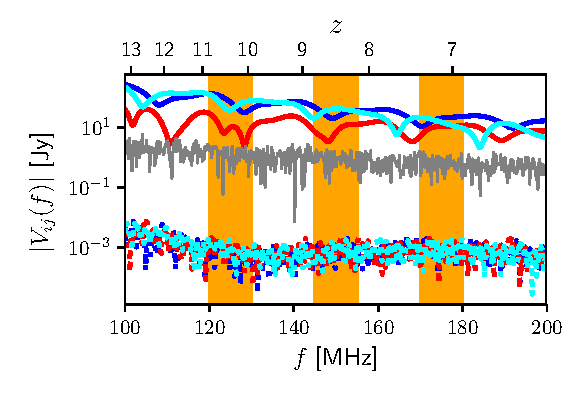
\includegraphics[width=\linewidth]{visamp_spectra_asm_eor_noise}
\caption{Spatial coherence amplitude spectra measured on three non-redundant 14.6~m antenna spacings are shown in red, blue and cyan. The solid lines show amplitudes from synchrotron from diffuse and compact foregrounds. The gray curve shows the typical noise obtained with 1~min integration. The dotted curves show spatial coherence amplitudes from EoR signal on these antenna spacings from a fiducial model obtained using 21cmFAST. Typically, the foregrounds are $\gtrsim 10^4$ times brighter than the EoR signal. The orange bands denote the frequency sub-bands centered on 125~MHz, 150~MHz, and 175~MHz each of 10~MHz effective bandwidth. \label{fig:vis-spectra}}
\end{figure}

Fig.~\ref{fig:cp-spectra} shows the spectra of the bi-spectrum phase, $\phi_\nabla$, for the foreground and EoR components separately. It is clear that the foreground contributions to $\phi_\nabla$ are characterized by a smoother spectrum whereas the EoR signal is rapidly fluctuating. Identifying with Eq.~\ref{eqn:cpphase-sum},
\begin{align}\label{eqn:cp-components}
  \phi_\nabla^\textrm{m} &= \left(\phi_\nabla^\textrm{F} + \delta\phi_\nabla^\textrm{H{\sc i}}\right) + \delta\phi_\nabla^\textrm{N}
\end{align}
where, the terms in the parenthesis are purely sky-based. $\delta\phi_\nabla^\textrm{H{\sc i}}$ and $\delta\phi_\nabla^\textrm{H{\sc i}}$ are to be interpreted as perturbations due to the \HI\ and noise fluctuations respectively, relative to the dominant phase from foregrounds, $\phi_\nabla^\textrm{F}$. Writing $V_{ij}^\textrm{m}=V_{ij}^\textrm{F}+V_{ij}^\textrm{H{\sc i}}+V_{ij}^\textrm{N}$, and when $V_{ij}^\textrm{F}$ dominates $V_{ij}^\textrm{m}$ ($\delta\phi_\nabla^\textrm{H{\sc i}}, \delta\phi_\nabla^\textrm{N} \ll 1$), $B_\nabla^\textrm{m}$ can be expanded to linear order in $V_{ij}^\textrm{H{\sc i}}$, $V_{ij}^\textrm{N}$, $\delta\phi_\nabla^\textrm{H{\sc i}}$ and $\delta\phi_\nabla^\textrm{N}$, and it can be shown that 
\begin{align}
  \Big|\delta\phi_\nabla^\textrm{H{\sc i}}\Big|^2 + \Big|\delta\phi_\nabla^\textrm{N}\Big|^2 &\approx \sum_{ij} \Big|\frac{V_{ij}^\textrm{H{\sc i}}}{V_{ij}^\textrm{F}}\Big|^2 + \Big|\frac{V_{ij}^\textrm{N}}{V_{ij}^\textrm{F}}\Big|^2,
\end{align}
where, $V_{ab}^\textrm{F}$ and $V_{ij}^\textrm{H{\sc i}}$ denote contributions from the foregrounds and the EoR \HI\ signal to the spatial coherence, respectively. Therefore, $\delta\phi_\nabla^\textrm{H{\sc i}}$ is effectively a measure of the EoR \HI\ line strength to foreground continuum ratio.

\begin{figure}[htb]
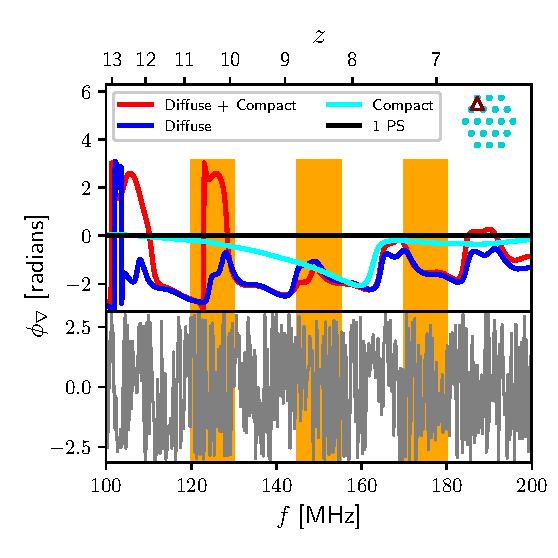
\includegraphics[width=0.85\linewidth]{closure_phase_spectra_0_1_8}
\caption{Bi-spectrum phase spectra of individual components in the sky model -- single point source (black) with $\phi_\nabla=0$, compact sources (cyan), diffuse foregrounds (blue), diffuse and compact components combined (red), and the EoR \HI\ fluctuations (gray) -- for a 14.6~m equilateral triad in the HERA-19 layout depicted in the upper right corner. The \HI\ component is highly fluctuating relative to the foregrounds. The phase wrap discontinuities at $\phi_\nabla=\pm \pi$ are not of a physical origin. The orange sub-bands are same as in Fig.~\ref{fig:vis-spectra}. \label{fig:cp-spectra}}
\end{figure}

\section{Extraction of the cosmic signal}\label{sec:extraction}

The different spectral characteristics -- smooth $\phi_\nabla^\textrm{F}$ and fluctuating $\delta\phi_\nabla^\textrm{H{\sc i}}$ -- indicate that techniques similar to the power spectrum approaches could be employed to separate the cosmic signal from foregrounds but avoiding the need for high-precision spectral calibration that most existing approaches rely on.

If a number of independent measurements are available, they could be used to average $\phi_\nabla^\textrm{m}$ to reduce the standard deviation of $\delta\phi_\nabla^\textrm{N}$ (noise uncertainty) by taking advantage of its Gaussian distribution. When $\delta\phi_\nabla^\textrm{N}$ is sufficiently low, $\delta\phi_\nabla^\textrm{H{\sc i}}$ will dominate the spectral fluctuations in $\phi_\nabla^\textrm{m}$, while $\phi_\nabla^\textrm{F}$ will be dominant overall but spectrally smooth. Then the standard deviation in $\phi_\nabla^\textrm{m}$ will be similar in form to Eq.~(\ref{eqn:cprms-noise}):
\begin{align}
  \sigma_{\phi_\nabla^\textrm{m}}^2 &= \sum_{ij}\, (\sqrt{2}\,\rho_{ij}^\textrm{H{\sc i}})^{-2}, \label{eqn:cprms-EoR}
\end{align}
where, $\rho_{ij}^\textrm{H{\sc i}} = |V_{ij}^\textrm{T}|/|V_{ij}^\textrm{H{\sc i}}| \approx |V_{ij}^\textrm{F}|/|V_{ij}^\textrm{H{\sc i}}|$. This approximation is valid because usually $\rho_{ij}^\textrm{H{\sc i}} \gtrsim 10^4 \gg 1$. 

Thus, when $\rho_{ij}^\textrm{H{\sc i}} < \rho_{ij}^\textrm{N}$, $\sigma_{\phi_\nabla^\textrm{m}}$ can be used to estimate $|V_{ij}^\textrm{F}|/|V_{ij}^\textrm{H{\sc i}}|$, which in turn can be used to infer $|V_{ij}^\textrm{H{\sc i}}|$ if $V_{ij}^\textrm{F}$ is known. $|V_{ij}^\textrm{H{\sc i}}|$ is directly related to the EoR H~{\sc i} brightness temperature fluctuations, $\langle(\delta T_\textrm{b}^\textrm{H{\sc i}})^2\rangle$, which can be inferred as a function of frequency, or redshift. This is discussed further in sections that follow.

\subsection{Delay Power Spectrum of Bi-spectrum Phase}\label{sec:cp-FG-wedge}

While any method that relies on separating a signal from contaminants using differences in spectral characteristics is applicable, we employ the {\it Delay Spectrum} approach \cite{par12a,par12b}. Since the $\phi_\nabla$ spectrum can have discontinuities at $\phi_\nabla=\pm\pi$, it can have non-physical spectral features. Hence, we define $\xi_\nabla = e^{i\phi_\nabla}$, which is unaffected by these discontinuities. We perform a delay transform:
\begin{align}\label{eqn:cpdspec}
  \Xi_\nabla(\tau) &= \int \xi_\nabla(f)\,W(f)\,e^{i2\pi f\tau}\,\mathrm{d}f,
\end{align}
where, $W(f)$ is a spectral weighting usually chosen to control the quality of the delay spectrum \citep{thy13,thy16} and has an effective bandwidth, $B_\textrm{eff}$. $\Xi_\nabla(\tau)$ has units of Hz. 

We define the delay cross-power spectrum of $\xi_\nabla(f)$ as:
\begin{align}
  P_\nabla(k_\parallel) &\equiv \mathfrak{Re}\bigg\{\Xi_\nabla(\tau)\,\Xi_{\nabla^\prime}^*(\tau)\bigg\} \left(\frac{\Delta D}{B_\textrm{eff}^2}\right), \label{eqn:delay-power-spectrum}
\end{align}
where, $\Delta D\equiv \Delta D(z)$ is the comoving depth along the line of sight corresponding to $B_\textrm{eff}$ at redshift $z$, $k_\parallel\approx 2\pi\tau B_\textrm{eff}/\Delta D$ is line-of-sight wavenumber, and $\mathfrak{Re}\{\cdot\}$ denotes the real part. In this paper, we use cosmological parameters from \cite{planck15xiii} with $H_0=100\,h$~km~s$^{-1}$~Mpc$^{-1}$. $P_\nabla(k_\parallel)$ is in units of $h^{-1}$~Mpc. When $\Xi_\nabla(\tau)=\Xi_{\nabla^\prime}(\tau)$, $P_\nabla(k_\parallel)$ reduces to delay auto-power spectrum. In \S\ref{sec:averaging}, we describe the usage of Eq.~(\ref{eqn:delay-power-spectrum}) in different contexts. 

From Eq.~(\ref{eqn:cpphase-sum}), since $\xi_\nabla = \prod_{ij} e^{i\phi_{ij}}$,
\begin{align}
\Xi_\nabla(\tau) &= \Xi_{ab}(\tau)\circledast \Xi_{bc}(\tau)\circledast \Xi_{ca}(\tau)\circledast \mathcal{W}(\tau), \label{eqn:cpdspec-convolution}
\end{align}
where, $\{\xi_{ij}(f),\,\Xi_{ij}(\tau)\}$, and $\{W(f),\,\mathcal{W}(\tau)\}$ are Fourier transform pairs, and $\circledast$ denotes convolution.  Foreground contribution to spatial coherence is known to be confined to delay modes within the {\it horizon limits} \cite{bow09,liu09,liu14a,liu14b,dat10,liu11,gho12,mor12,par12b,tro12,ved12,dil13,pob13,thy13,thy15a,thy15b,thy16,dil14}. Since $\Xi_\nabla(\tau)$ results from the convolution of the delay spectrum responses of the spatial coherence phases, the foreground contribution to $\Xi_\nabla(\tau)$ is expected to be more extended along $\tau$ (and $k_\parallel$) relative to $\Xi_{ij}(\tau)$. This relation will be explored in a forthcoming study. 

\subsection{Improving signal to noise in measurements}\label{sec:averaging}

We require $\sigma_{\phi_\nabla^\textrm{H{\sc i}}} > \sigma_{\phi_\nabla^\textrm{N}}$ such that $\phi_\nabla^\textrm{F}, \delta\phi_\nabla^\textrm{H{\sc i}} > \delta\phi_\nabla^\textrm{N}$ in order to detect EoR and estimate $\rho_{ab}^\textrm{H{\sc i}}$. This can be achieved by a combination of the following.

First, $\phi_\nabla^\textrm{m}$ can be averaged coherently until the variation due to the transiting sky exceeds the decrease in noise due to averaging \cite{car18}. An Allan Variance estimate for HERA showed this timescale to be $\lesssim 2$~min \cite{car18}.

Second, $\phi_\nabla^\textrm{m}$ can be averaged across multiple days at a fixed LST before computing $P_\nabla(k_\parallel)$, as long as the array size is small compared to the predominant spatial scales in the ionospheric variations, as has been observed to be the case for HERA \cite{car18}. 

Third, the measurements of redundant triads can be averaged coherently in $\phi_\nabla^\textrm{m}$, before computing the power spectrum.  For non-redundant triads, it may be possible to average incoherently in $P_\nabla(k_\parallel)$, using  $\Xi_\nabla(\tau)$ and $\Xi_{\nabla^\prime}^*(\tau)$ from triad pairs $\nabla$ and $\nabla^\prime$ respectively. Measurements across more triad classes -- equilateral, isosceles, and scalene -- and baseline lengths, could be used to average incoherently in power spectrum to further improve sensitivity analogous to power spectrum approaches. 

Lastly, for measurements spaced in time larger than the coherence timescale,  since the EoR signal is statistically isotropic in space while the foregrounds are not, such measurements can be used to first compute the individual delay cross-power spectra, $P_\nabla(k_\parallel)$, pairwise across temporally spaced measurements $\Xi_\nabla(\tau)$ and $\Xi_{\nabla^\prime}^*(\tau)$ and then be averaged incoherently. 

\subsection{Detection of Cosmic Reionization}\label{sec:EoR-detection}

The primary application of this technique is to detect the EoR \HI\ signal. We consider the spectral band 100--200~MHz divided into 512 spectral channels, each 195.3125~kHz wide. Using an {\it Airy} power pattern for the HERA dish, we used PRISim \footnote{PRISim is the open source Precision Radio Interferometry Simulator Python package available at \href{https://github.com/nithyanandan/PRISim}{https://github.com/nithyanandan/PRISim}.} to simulate the synchrotron foregrounds, an EoR model, and noise as described in \S\ref{sec:modeling} and obtain $V_{ij}^\textrm{F}(f)$, $V_{ij}^\textrm{H{\sc i}}(f)$, and $V_{ij}^\textrm{N}(f)$, on various antenna spacings for a conservative phase-coherent integration interval of 1~min (see \S\ref{sec:averaging}) \cite{car18}. 

For bi-spectrum phase, we consider 14.6~m equilateral antenna triads and assume ideal redundancy for the array. The total number of such measurements is assumed to be $N_\textrm{m} \sim 10^6$ (after allowing for $\sim$~50\% efficiency of data quality from $\sim 30$ redundant 14.6~m equilateral triads with HERA-47, $\sim$~8~hours of observing per day at 1~min integration intervals, repeated over $\sim$~150 nights). For each of these measurements, $\delta\phi_\nabla^\textrm{N}$ was drawn from a Gaussian distribution using $\sigma_{\phi_\nabla^\textrm{N}}$ in Eq.~(\ref{eqn:cprms-noise}). As various combinations of coherent and incoherent averaging depend on the specific instrument characteristics, we keep this analysis generic by assuming there are $N_\textrm{c}$ coherent measurements of $\phi_\nabla^\textrm{m}$ and for each of these measurements, there are $N_\textrm{ic}$ incoherent measurements such that $N_\textrm{c}N_\textrm{ic}=N_\textrm{m}$. $\phi_\nabla^\textrm{m}$ is averaged coherently over $N_\textrm{c}$ measurements, and then averaged incoherently in $P_\nabla(k_\parallel)$ measured for all incoherent pairs of $\phi_\nabla^\textrm{m}$. For computing $\Xi_\nabla(\tau)$, we choose $W(f)$ by applying inverse Fourier transform of the squared delay response of a {\it Blackman-Harris} spectral weighting \cite{har78} as proposed in \cite{thy16}, using sub-bands centered at 125~MHz, 150~MHz, and 175~MHz, with an effective bandwidth of $B_\textrm{eff}\simeq 10$~MHz (to minimize EoR signal evolution over the redshift range).

Fig.~\ref{fig:cpdps} shows the delay cross-power spectra, $P_\nabla(k_\parallel)$, of $\phi_\nabla^\textrm{m}$ obtained for the three sub-bands, with an initial S/N, $\rho_{ij}^\textrm{N}=200$. At $|k_\parallel| \gtrsim 0.5\,h$~Mpc$^{-1}$, the contributions from the cosmological \HI\ fluctuations, $\delta\phi_\nabla^\textrm{H{\sc i}}$ (in gray and black), dominate over $\phi_\nabla^\textrm{F} + \delta\phi_\nabla^\textrm{N}$ in the 150~MHz and 175~MHz sub-bands. The use of cross-power delay spectrum removes the noise bias and results in occasional negative values in the presence of noise. It also shows that $N_\textrm{m}$ used in this example is sufficient to make $\rho_{ij}^\textrm{H{\sc i}} < \rho_{ij}^\textrm{N}$ and the EoR signal detectable in individual line-of-sight modes, $|k_\parallel| \gtrsim 0.5\,h$~Mpc$^{-1}$. The absence of a clear detection in the 125~MHz sub-band is discussed below.

\begin{figure*}[htb]
  \subfloat[][125~MHz sub-band ($z\approx 10.4$)]{\label{fig:cpdps-125}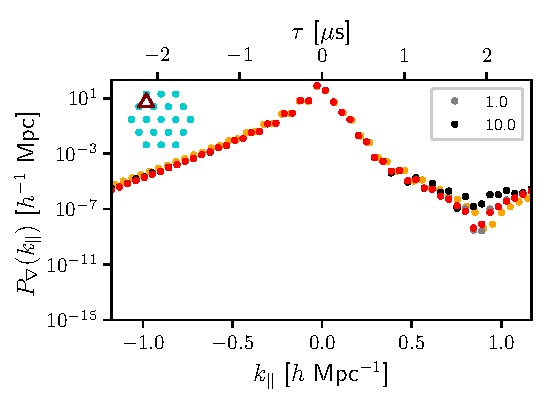
\includegraphics[width=0.32\linewidth]{cpdps_125MHz_SNR_200_nsamples_1048576}}
  \subfloat[][150~MHz sub-band ($z\approx 8.5$)]{\label{fig:cpdps-150}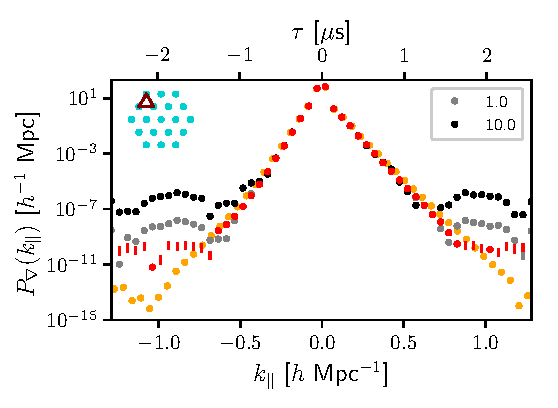
\includegraphics[width=0.32\linewidth]{cpdps_150MHz_SNR_200_nsamples_1048576}}
  \subfloat[][175~MHz sub-band ($z\approx 7.1$)]{\label{fig:cpdps-175}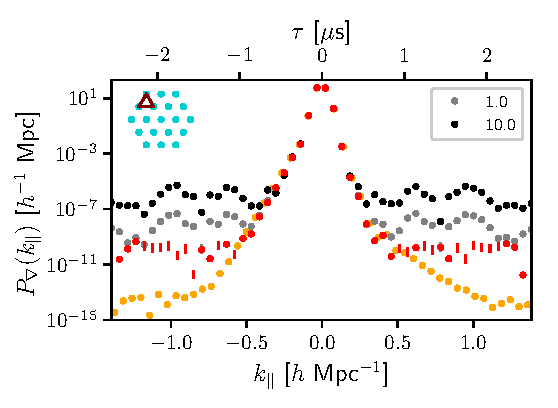
\includegraphics[width=0.32\linewidth]{cpdps_175MHz_SNR_200_nsamples_1048576}}
\caption{Delay power spectra of simulated bi-spectrum phases in sub-bands centered at 125~MHz (left), 150~MHz (middle), and 175~MHz (right) that include contributions from foregrounds, EoR signal, and thermal noise. The red curve denotes when only foregrounds are present, $\phi_\nabla^\textrm{m}=\phi_\nabla^\textrm{F}$. The anisotropic foreground model employed \cite{thy15a} results in the asymmetry around $k_\parallel=0\,h^{-1}$~Mpc. The orange curve is for thermal noise superimposed on the foreground component, $\phi_\nabla^\textrm{m}=\phi_\nabla^\textrm{F}+\delta\phi_\nabla^\textrm{N}$, after averaging $N_\textrm{m} \sim 10^6$ measurements. The gray curve is when contribution from a fiducial EoR model is also present, $\phi_\nabla^\textrm{m}=\phi_\nabla^\textrm{F}+\delta\phi_\nabla^\textrm{H{\sc i}}+\delta\phi_\nabla^\textrm{N}$, after averaging same number of measurements. The black curve is the same as the gray one except the fiducial EoR model is 10 times stronger in intensity. The dot and vertical markers denote positive and negative values respectively. The latter are a result of removal of noise bias obtained by using cross-power spectra (Eq.~\ref{eqn:delay-power-spectrum}). With sufficient mitigation of $\delta\phi_\nabla^\textrm{N}$, the EoR \HI\ contribution is significantly detectable at $|k_\parallel| \gtrsim 0.5\,h$~Mpc$^{-1}$ at $z\approx 8.5$ and $z\approx 7.1$. At $z\approx 10.4$, the EoR contribution is virtually inseparable from the foregrounds because the foregrounds are brighter and the EoR signal is weaker \cite[][see power spectrum amplitude of {\sc faint galaxies} model at $k=0.5$~Mpc$^{-1}$ in their Fig.~2]{gre17b}. The detection significance is noted to depend on the strength of EoR H~{\sc i} emission relative to the foregrounds. An increase in EoR strength by a factor of 10 shows $\sim 100$-fold increase in $P_\nabla(k_\parallel)$ in $|k_\parallel| \gtrsim 0.5\,h$~Mpc$^{-1}$ at $z\approx 8.5$ and $z\approx 7.1$, indicating its sensitive dependence on $\rho_{ij}^\textrm{H{\sc i}}$. In essence, the measurement represents a line-to-continuum ratio, such that the cosmological EoR H~{\sc i} brightness temperature fluctuations, $\langle(\delta T_\textrm{b}^\textrm{H{\sc i}}(z))^2\rangle$, can be inferred if a reliable foreground model is available. \label{fig:cpdps}}
\end{figure*}

\subsection{EoR H~{\sc i} Brightness Temperature Fluctuations} \label{sec:Tb-variance}

Beyond simple detection, we need to estimate the EoR \HI\ brightness temperature fluctuations, $\langle(\delta T_\textrm{b}^\textrm{H{\sc i}}(z))^2\rangle$, in various sub-bands using the separation in $P_\nabla(k_\parallel)$, demonstrated above. When $\rho_{ij}^\textrm{H{\sc i}} < \rho_{ij}^\textrm{N}$, the separation between $\phi_\nabla^\textrm{m}$ (black or gray) and $\phi_\nabla^\textrm{F} + \delta\phi_\nabla^\textrm{N}$ (red) in $P_\nabla(k_\parallel)$ depends sensitively on $\rho_{ab}^\textrm{H{\sc i}}$.

Fig.~\ref{fig:cpdps} shows $P_\nabla(k_\parallel)$ for the three sub-bands for different values of simulated $\langle(\delta T_\textrm{b}^\textrm{H{\sc i}}(z))^2\rangle$, or equivalently $\rho_{ij}^\textrm{H{\sc i}}$, while the foreground model was unaltered in each sub-band. As the strength of the EoR \HI\ component increases (ten-fold in $\langle(\delta T_\textrm{b}^\textrm{H{\sc i}}(z))^2\rangle^{1/2}$), the separation in $P_\nabla(k_\parallel)$ also increases at $|k_\parallel| \gtrsim 0.5\,h$~Mpc$^{-1}$ ($\sim 100$ times), most clearly in the 150~MHz and 175~MHz sub-bands. Conversely, based on this separation in delay spectrum, $\rho_{ij}^\textrm{H{\sc i}}$ can be estimated in the different sub-bands, or redshift ranges, which in turn can be used to estimate $\langle(\delta T_\textrm{b}^\textrm{H{\sc i}}(z))^2\rangle$ by using the best foreground models available in the different sub-bands. The accuracy of $\langle(\delta T_\textrm{b}^\textrm{H{\sc i}}(z))^2\rangle$ so determined will depend on the uncertainty in the foreground model, which is not required to be as precise as the calibration requirement.

The redshift evolution of separability in $P_\nabla(k_\parallel)$ depends on relative strengths of the foreground and the EoR \HI\ signal. In the 175~MHz sub-band ($z\approx 7.1$), relative to the 150~MHz sub-band ($z\approx 8.5$), $\langle(\delta T_\textrm{b}^\textrm{H{\sc i}}(z))^2\rangle$ is weaker (based on the fiducial {\sc faint galaxies} model at $k=0.5$~Mpc$^{-1}$ in Fig.~2 of \cite{gre17b}) but the foreground synchrotron temperature is also fainter roughly by the same factor. Therefore, the separability of EoR \HI\ in $P_\nabla(k_\parallel)$ is roughly similar in the two sub-bands (Fig.~\ref{fig:cpdps-150}, \ref{fig:cpdps-175}). However, in the 125~MHz sub-band ($z\approx 10.4$), $\langle(\delta T_\textrm{b}^\textrm{H{\sc i}}(z))^2\rangle$ in the fiducial EoR model is fainter whereas the foreground temperature is larger, thereby significantly decreasing the relative spectral contrast between foregrounds and the EoR signal. Hence, a clear separability is not seen in $P_\nabla(k_\parallel)$ at $z\approx 10.4$ (Fig.~\ref{fig:cpdps-125}).

A direct confirmation of this hypothesis can be obtained by estimating $\rho_{ij}^\textrm{H{\sc i}}$ in different sub-bands and verifying that there is no separation in $P_\nabla(k_\parallel)$ at $|k_\parallel| \gtrsim 0.5\,h$~Mpc$^{-1}$ at $z\lesssim 6$, when the IGM is understood to be fully ionized, with a reasoning similar to \cite{pob16b}. This will correspond to $(\rho_{ij}^\textrm{H{\sc i}})^{-1} \ll 1$. Lack of separation in $P_\nabla(k_\parallel)$, such as at $z\approx 10.4$, will enable placing upper limits on $\langle (\delta T_\textrm{b}^\textrm{H{\sc i}}(z))^2\rangle$.

% The presence of strong foregrounds relative to thermal noise (high $\rho_{ij}^\textrm{N}$) provides a reliable phase reference (small $\sigma_\nabla^\textrm{N}$) and thus requires fewer $N_\textrm{m}$ to mitigate thermal noise contributions. However, as seen from Fig.~\ref{fig:cpdps}, the presence of strong foregrounds relative to EoR fluctuations (high $\rho_{ij}^\textrm{\HI}$) implies the dynamic range to be achieved for EoR detection is correspondingly high and is possible only at $|k_\parallel| \gtrsim 0.5\,h$~Mpc$^{-1}$. If the foregrounds were instead weaker, they will not serve as a strong phase reference. Hence, mitigating thermal noise contributions may require larger $N_\textrm{m}$, but a lower dynamic range may be sufficient for a detection and more $k_\parallel$-modes may be available due to lowered spillover contamination, thereby increasing the effective sensitivity to the EoR signal. 

\subsection{Prospects and Challenges}\label{sec:prospects-challenges}

Beyond the simple demonstration of our approach presented here, there are many ways to improve the prospects of detecting the cosmic reionization signal using the bi-spectrum phase, particularly in the context of a redundant array such as HERA (though it applies to non-redundant arrays as well). HERA, upon completion, will consist of 350 antennas yielding $\sim$~10--100 times more measurements than used in this analysis, and could thereby go deeper in overall sensitivity. Cylindrical or spherical bins in different $k$-modes (including different triad classes) can be weighted optimally \cite{liu14a,liu14b,dil15} to maximize sensitivity. Removal of the foreground contribution, $\xi_\nabla^\textrm{F}$, in $\xi_\nabla^\textrm{m}$ could potentially relax the dynamic range required for detection and boost sensitivity in $|k_\parallel| \lesssim 0.5\,h$~Mpc$^{-1}$.

Challenges to this approach arise from effects that introduce systematic spectral errors in Eq.~(\ref{eqn:cp-components}). Due to the triple convolution in Eq.~(\ref{eqn:cpdspec-convolution}), there may be  fewer sensitive $k_\parallel$-modes. Presence of significant baseline-based gain terms, off-diagonal terms in the direction-independent Jones matrix of an antenna indicative of polarization leakage between the dual-polarization feeds, and direction-dependent antenna gain terms will introduce systematic departures from Eq.~(\ref{eqn:cp-components}). Excision of radio frequency interference (RFI) affected frequencies, if not carefully corrected for, will introduce spectral artifacts, contaminate the relatively foreground-free $k_\parallel$-modes, and reduce sensitivity. It must be noted that most existing approaches face these challenges as well.

\section{Summary}\label{sec:summary}

A primary limitation to existing low-frequency EoR 21~cm cosmology experiments remains high-precision spectral calibration in order to remove the strong continuum foregrounds. We propose a new approach that uses bi-spectrum phase, which represents an intrinsic property of the sky and is thus impervious to antenna-based calibration and associated errors, unlike existing approaches.
  
The primary goal of the proposed technique is to obtain an interferometric detection of the \HI\ 21~cm signal from the neutral IGM during cosmic reionization. The next goal will be to relate the measured EoR \HI\ bi-spectrum phase power spectrum to the astrophysical quantities of interest, particularly, the brightness temperature fluctuations. The magnitude of the line signal relative to that of the foreground continuum in the bi-spectrum phase power spectrum, is essentially a measure of the line-to-continuum ratio, since the line signal introduces small, frequency-dependent, perturbations on the phase of the spatial coherence. Hence, the line signal strength can be calibrated against a foreground model.

Ultimately, the quantitative interpretation will entail a standard forward-modeling process, comparing measurements to the predictions of bi-spectrum phase power spectra for different sky models. This work investigates one such realization, to demonstrate that a quantitative relationship exists between the EoR signal strength and the bi-spectrum phase power spectra.

% Our study has used a highly redundant array, but the approach is applicable to non-redundant arrays too. This paper is an exposition of the basic approach to \HI\ 21~cm cosmology using the spectral response in the bi-spectrum phase. 

In future work, we will investigate the challenges listed above, such as RFI flagging and baseline-dependent responses, using the HERA data.

\begin{acknowledgments}
We acknowledge the insightful and helpful inputs from Gianni Bernardi, Judd Bowman, James Aguirre, Aaron Parsons, Jonathan Pober, Adam Beardsley, and Peter Williams that helped in the preparation of this manuscript. The National Radio Astronomy Observatory is a facility of the National Science Foundation operated under cooperative agreement by Associated Universities, Inc. We acknowledge support from the Royal Society and the Newton Fund under grant NA150184.
\end{acknowledgments}

% \subsection{\label{sec:level2}Second-level heading: Formatting}

% This file may be formatted in either the \texttt{preprint} or
% \texttt{reprint} style. \texttt{reprint} format mimics final journal output. 
% Either format may be used for submission purposes. \texttt{letter} sized paper should
% be used when submitting to APS journals.

% \subsubsection{Wide text (A level-3 head)}
% The \texttt{widetext} environment will make the text the width of the
% full page, as on page~\pageref{eq:wideeq}. (Note the use the
% \verb+\pageref{#1}+ command to refer to the page number.) 
% \paragraph{Note (Fourth-level head is run in)}
% The width-changing commands only take effect in two-column formatting. 
% There is no effect if text is in a single column.

% \subsection{\label{sec:citeref}Citations and References}
% A citation in text uses the command \verb+\cite{#1}+ or
% \verb+\onlinecite{#1}+ and refers to an entry in the bibliography. 
% An entry in the bibliography is a reference to another document.

% \subsubsection{Citations}
% Because REV\TeX\ uses the \verb+natbib+ package of Patrick Daly, 
% the entire repertoire of commands in that package are available for your document;
% see the \verb+natbib+ documentation for further details. Please note that
% REV\TeX\ requires version 8.31a or later of \verb+natbib+.

% \paragraph{Syntax}
% The argument of \verb+\cite+ may be a single \emph{key}, 
% or may consist of a comma-separated list of keys.
% The citation \emph{key} may contain 
% letters, numbers, the dash (-) character, or the period (.) character. 
% New with natbib 8.3 is an extension to the syntax that allows for 
% a star (*) form and two optional arguments on the citation key itself.
% The syntax of the \verb+\cite+ command is thus (informally stated)
% \begin{quotation}\flushleft\leftskip1em
% \verb+\cite+ \verb+{+ \emph{key} \verb+}+, or\\
% \verb+\cite+ \verb+{+ \emph{optarg+key} \verb+}+, or\\
% \verb+\cite+ \verb+{+ \emph{optarg+key} \verb+,+ \emph{optarg+key}\ldots \verb+}+,
% \end{quotation}\noindent
% where \emph{optarg+key} signifies 
% \begin{quotation}\flushleft\leftskip1em
% \emph{key}, or\\
% \texttt{*}\emph{key}, or\\
% \texttt{[}\emph{pre}\texttt{]}\emph{key}, or\\
% \texttt{[}\emph{pre}\texttt{]}\texttt{[}\emph{post}\texttt{]}\emph{key}, or even\\
% \texttt{*}\texttt{[}\emph{pre}\texttt{]}\texttt{[}\emph{post}\texttt{]}\emph{key}.
% \end{quotation}\noindent
% where \emph{pre} and \emph{post} is whatever text you wish to place 
% at the beginning and end, respectively, of the bibliographic reference
% (see Ref.~[\onlinecite{witten2001}] and the two under Ref.~[\onlinecite{feyn54}]).
% (Keep in mind that no automatic space or punctuation is applied.)
% It is highly recommended that you put the entire \emph{pre} or \emph{post} portion 
% within its own set of braces, for example: 
% \verb+\cite+ \verb+{+ \texttt{[} \verb+{+\emph{text}\verb+}+\texttt{]}\emph{key}\verb+}+.
% The extra set of braces will keep \LaTeX\ out of trouble if your \emph{text} contains the comma (,) character.

% The star (*) modifier to the \emph{key} signifies that the reference is to be 
% merged with the previous reference into a single bibliographic entry, 
% a common idiom in APS and AIP articles (see below, Ref.~[\onlinecite{epr}]). 
% When references are merged in this way, they are separated by a semicolon instead of 
% the period (full stop) that would otherwise appear.

% \paragraph{Eliding repeated information}
% When a reference is merged, some of its fields may be elided: for example, 
% when the author matches that of the previous reference, it is omitted. 
% If both author and journal match, both are omitted.
% If the journal matches, but the author does not, the journal is replaced by \emph{ibid.},
% as exemplified by Ref.~[\onlinecite{epr}]. 
% These rules embody common editorial practice in APS and AIP journals and will only
% be in effect if the markup features of the APS and AIP Bib\TeX\ styles is employed.

% \paragraph{The options of the cite command itself}
% Please note that optional arguments to the \emph{key} change the reference in the bibliography, 
% not the citation in the body of the document. 
% For the latter, use the optional arguments of the \verb+\cite+ command itself:
% \verb+\cite+ \texttt{*}\allowbreak
% \texttt{[}\emph{pre-cite}\texttt{]}\allowbreak
% \texttt{[}\emph{post-cite}\texttt{]}\allowbreak
% \verb+{+\emph{key-list}\verb+}+.

% \subsubsection{Example citations}
% By default, citations are numerical\cite{Beutler1994}.
% Author-year citations are used when the journal is RMP. 
% To give a textual citation, use \verb+\onlinecite{#1}+: 
% Refs.~\onlinecite{[][{, and references therein}]witten2001,Bire82}. 
% By default, the \texttt{natbib} package automatically sorts your citations into numerical order and ``compresses'' runs of three or more consecutive numerical citations.
% REV\TeX\ provides the ability to automatically change the punctuation when switching between journal styles that provide citations in square brackets and those that use a superscript style instead. This is done through the \texttt{citeautoscript} option. For instance, the journal style \texttt{prb} automatically invokes this option because \textit{Physical 
% Review B} uses superscript-style citations. The effect is to move the punctuation, which normally comes after a citation in square brackets, to its proper position before the superscript. 
% To illustrate, we cite several together 
% \cite{[See the explanation of time travel in ]feyn54,*[The classical relativistic treatment of ][ is a relative classic]epr,witten2001,Berman1983,Davies1998,Bire82}, 
% and once again in different order (Refs.~\cite{epr,feyn54,Bire82,Berman1983,witten2001,Davies1998}). 
% Note that the citations were both compressed and sorted. Futhermore, running this sample file under the \texttt{prb} option will move the punctuation to the correct place.

% When the \verb+prb+ class option is used, the \verb+\cite{#1}+ command
% displays the reference's number as a superscript rather than in
% square brackets. Note that the location of the \verb+\cite{#1}+
% command should be adjusted for the reference style: the superscript
% references in \verb+prb+ style must appear after punctuation;
% otherwise the reference must appear before any punctuation. This
% sample was written for the regular (non-\texttt{prb}) citation style.
% The command \verb+\onlinecite{#1}+ in the \texttt{prb} style also
% displays the reference on the baseline.

% \subsubsection{References}
% A reference in the bibliography is specified by a \verb+\bibitem{#1}+ command
% with the same argument as the \verb+\cite{#1}+ command.
% \verb+\bibitem{#1}+ commands may be crafted by hand or, preferably,
% generated by Bib\TeX. 
% REV\TeX~4.1 includes Bib\TeX\ style files
% \verb+apsrev4-1.bst+, \verb+apsrmp4-1.bst+ appropriate for
% \textit{Physical Review} and \textit{Reviews of Modern Physics},
% respectively. To display titles for cited journal articles, use the \texttt{longbibliography} class option.

% \subsubsection{Example references}
% This sample file employs the \verb+\bibliography+ command, 
% which formats the \texttt{\jobname .bbl} file
% and specifies which bibliographic databases are to be used by Bib\TeX\ 
% (one of these should be by arXiv convention \texttt{\jobname .bib}).
% Running Bib\TeX\ (via \texttt{bibtex \jobname}) 
% after the first pass of \LaTeX\ produces the file
% \texttt{\jobname .bbl} which contains the automatically formatted
% \verb+\bibitem+ commands (including extra markup information via
% \verb+\bibinfo+ and \verb+\bibfield+ commands). 
% If not using Bib\TeX, you will have to create the \verb+thebibiliography+ environment 
% and its \verb+\bibitem+ commands by hand.

% Numerous examples of the use of the APS bibliographic entry types appear in the bibliography of this sample document.
% You can refer to the \texttt{\jobname .bib} file, 
% and compare its information to the formatted bibliography itself.

% \subsection{Footnotes}%
% Footnotes, produced using the \verb+\footnote{#1}+ command, 
% usually integrated into the bibliography alongside the other entries.
% Numerical citation styles do this%
% \footnote{Automatically placing footnotes into the bibliography requires using BibTeX to compile the bibliography.};
% author-year citation styles place the footnote at the bottom of the text column.
% Note: due to the method used to place footnotes in the bibliography, 
% \emph{you must re-run Bib\TeX\ every time you change any of your document's footnotes}. 

% \section{Math and Equations}
% Inline math may be typeset using the \verb+$+ delimiters. Bold math
% symbols may be achieved using the \verb+bm+ package and the
% \verb+\bm{#1}+ command it supplies. For instance, a bold $\alpha$ can
% be typeset as \verb+$\bm{\alpha}$+ giving $\bm{\alpha}$. Fraktur and
% Blackboard (or open face or double struck) characters should be
% typeset using the \verb+\mathfrak{#1}+ and \verb+\mathbb{#1}+ commands
% respectively. Both are supplied by the \texttt{amssymb} package. For
% example, \verb+$\mathbb{R}$+ gives $\mathbb{R}$ and
% \verb+$\mathfrak{G}$+ gives $\mathfrak{G}$

% In \LaTeX\ there are many different ways to display equations, and a
% few preferred ways are noted below. Displayed math will center by
% default. Use the class option \verb+fleqn+ to flush equations left.

% Below we have numbered single-line equations; this is the most common
% type of equation in \textit{Physical Review}:
% \begin{eqnarray}
% \chi_+(p)\alt{\bf [}2|{\bf p}|(|{\bf p}|+p_z){\bf ]}^{-1/2}
% \left(
% \begin{array}{c}
% |{\bf p}|+p_z\\
% px+ip_y
% \end{array}\right)\;,
% \\
% \left\{%
%  \openone234567890abc123\alpha\beta\gamma\delta1234556\alpha\beta
%  \frac{1\sum^{a}_{b}}{A^2}%
% \right\}%
% \label{eq:one}.
% \end{eqnarray}
% Note the open one in Eq.~(\ref{eq:one}).

% Not all numbered equations will fit within a narrow column this
% way. The equation number will move down automatically if it cannot fit
% on the same line with a one-line equation:
% \begin{equation}
% \left\{
%  ab12345678abc123456abcdef\alpha\beta\gamma\delta1234556\alpha\beta
%  \frac{1\sum^{a}_{b}}{A^2}%
% \right\}.
% \end{equation}

% When the \verb+\label{#1}+ command is used [cf. input for
% Eq.~(\ref{eq:one})], the equation can be referred to in text without
% knowing the equation number that \TeX\ will assign to it. Just
% use \verb+\ref{#1}+, where \verb+#1+ is the same name that used in
% the \verb+\label{#1}+ command.

% Unnumbered single-line equations can be typeset
% using the \verb+\[+, \verb+\]+ format:
% \[g^+g^+ \rightarrow g^+g^+g^+g^+ \dots ~,~~q^+q^+\rightarrow
% q^+g^+g^+ \dots ~. \]


% \subsection{Multiline equations}

% Multiline equations are obtained by using the \verb+eqnarray+
% environment.  Use the \verb+\nonumber+ command at the end of each line
% to avoid assigning a number:
% \begin{eqnarray}
% {\cal M}=&&ig_Z^2(4E_1E_2)^{1/2}(l_i^2)^{-1}
% \delta_{\sigma_1,-\sigma_2}
% (g_{\sigma_2}^e)^2\chi_{-\sigma_2}(p_2)\nonumber\\
% &&\times
% [\epsilon_jl_i\epsilon_i]_{\sigma_1}\chi_{\sigma_1}(p_1),
% \end{eqnarray}
% \begin{eqnarray}
% \sum \vert M^{\text{viol}}_g \vert ^2&=&g^{2n-4}_S(Q^2)~N^{n-2}
%         (N^2-1)\nonumber \\
%  & &\times \left( \sum_{i<j}\right)
%   \sum_{\text{perm}}
%  \frac{1}{S_{12}}
%  \frac{1}{S_{12}}
%  \sum_\tau c^f_\tau~.
% \end{eqnarray}
% \textbf{Note:} Do not use \verb+\label{#1}+ on a line of a multiline
% equation if \verb+\nonumber+ is also used on that line. Incorrect
% cross-referencing will result. Notice the use \verb+\text{#1}+ for
% using a Roman font within a math environment.

% To set a multiline equation without \emph{any} equation
% numbers, use the \verb+\begin{eqnarray*}+,
% \verb+\end{eqnarray*}+ format:
% \begin{eqnarray*}
% \sum \vert M^{\text{viol}}_g \vert ^2&=&g^{2n-4}_S(Q^2)~N^{n-2}
%         (N^2-1)\\
%  & &\times \left( \sum_{i<j}\right)
%  \left(
%   \sum_{\text{perm}}\frac{1}{S_{12}S_{23}S_{n1}}
%  \right)
%  \frac{1}{S_{12}}~.
% \end{eqnarray*}

% To obtain numbers not normally produced by the automatic numbering,
% use the \verb+\tag{#1}+ command, where \verb+#1+ is the desired
% equation number. For example, to get an equation number of
% (\ref{eq:mynum}),
% \begin{equation}
% g^+g^+ \rightarrow g^+g^+g^+g^+ \dots ~,~~q^+q^+\rightarrow
% q^+g^+g^+ \dots ~. \tag{2.6$'$}\label{eq:mynum}
% \end{equation}

% \paragraph{A few notes on \texttt{tag}s} 
% \verb+\tag{#1}+ requires the \texttt{amsmath} package. 
% Place the \verb+\tag{#1}+ command before the \verb+\label{#1}+, if any. 
% The numbering produced by \verb+\tag{#1}+ \textit{does not affect} 
% the automatic numbering in REV\TeX; 
% therefore, the number must be known ahead of time, 
% and it must be manually adjusted if other equations are added. 
% \verb+\tag{#1}+ works with both single-line and multiline equations. 
% \verb+\tag{#1}+ should only be used in exceptional cases---%
% do not use it to number many equations in your paper. 
% Please note that this feature of the \texttt{amsmath} package
% is \emph{not} compatible with the \texttt{hyperref} (6.77u) package.

% Enclosing display math within
% \verb+\begin{subequations}+ and \verb+\end{subequations}+ will produce
% a set of equations that are labeled with letters, as shown in
% Eqs.~(\ref{subeq:1}) and (\ref{subeq:2}) below.
% You may include any number of single-line and multiline equations,
% although it is probably not a good idea to follow one display math
% directly after another.
% \begin{subequations}
% \label{eq:whole}
% \begin{eqnarray}
% {\cal M}=&&ig_Z^2(4E_1E_2)^{1/2}(l_i^2)^{-1}
% (g_{\sigma_2}^e)^2\chi_{-\sigma_2}(p_2)\nonumber\\
% &&\times
% [\epsilon_i]_{\sigma_1}\chi_{\sigma_1}(p_1).\label{subeq:2}
% \end{eqnarray}
% \begin{equation}
% \left\{
%  abc123456abcdef\alpha\beta\gamma\delta1234556\alpha\beta
%  \frac{1\sum^{a}_{b}}{A^2}
% \right\},\label{subeq:1}
% \end{equation}
% \end{subequations}
% Giving a \verb+\label{#1}+ command directly after the \verb+\begin{subequations}+, 
% allows you to reference all the equations in the \texttt{subequations} environment. 
% For example, the equations in the preceding subequations environment were
% Eqs.~(\ref{eq:whole}).

% \subsubsection{Wide equations}
% The equation that follows is set in a wide format, i.e., it spans the full page. 
% The wide format is reserved for long equations
% that cannot easily be set in a single column:
% \begin{widetext}
% \begin{equation}
% {\cal R}^{(\text{d})}=
%  g_{\sigma_2}^e
%  \left(
%    \frac{[\Gamma^Z(3,21)]_{\sigma_1}}{Q_{12}^2-M_W^2}
%   +\frac{[\Gamma^Z(13,2)]_{\sigma_1}}{Q_{13}^2-M_W^2}
%  \right)
%  + x_WQ_e
%  \left(
%    \frac{[\Gamma^\gamma(3,21)]_{\sigma_1}}{Q_{12}^2-M_W^2}
%   +\frac{[\Gamma^\gamma(13,2)]_{\sigma_1}}{Q_{13}^2-M_W^2}
%  \right)\;. 
%  \label{eq:wideeq}
% \end{equation}
% \end{widetext}
% This is typed to show how the output appears in wide format.
% (Incidentally, since there is no blank line between the \texttt{equation} environment above 
% and the start of this paragraph, this paragraph is not indented.)

% \section{Cross-referencing}
% REV\TeX{} will automatically number such things as
% sections, footnotes, equations, figure captions, and table captions. 
% In order to reference them in text, use the
% \verb+\label{#1}+ and \verb+\ref{#1}+ commands. 
% To reference a particular page, use the \verb+\pageref{#1}+ command.

% The \verb+\label{#1}+ should appear 
% within the section heading, 
% within the footnote text, 
% within the equation, or 
% within the table or figure caption. 
% The \verb+\ref{#1}+ command
% is used in text at the point where the reference is to be displayed.  
% Some examples: Section~\ref{sec:level1} on page~\pageref{sec:level1},
% Table~\ref{tab:table1},%
% \begin{table}[b]%The best place to locate the table environment is directly after its first reference in text
% \caption{\label{tab:table1}%
% A table that fits into a single column of a two-column layout. 
% Note that REV\TeX~4 adjusts the intercolumn spacing so that the table fills the
% entire width of the column. Table captions are numbered
% automatically. 
% This table illustrates left-, center-, decimal- and right-aligned columns,
% along with the use of the \texttt{ruledtabular} environment which sets the 
% Scotch (double) rules above and below the alignment, per APS style.
% }
% \begin{ruledtabular}
% \begin{tabular}{lcdr}
% \textrm{Left\footnote{Note a.}}&
% \textrm{Centered\footnote{Note b.}}&
% \multicolumn{1}{c}{\textrm{Decimal}}&
% \textrm{Right}\\
% \colrule
% 1 & 2 & 3.001 & 4\\
% 10 & 20 & 30 & 40\\
% 100 & 200 & 300.0 & 400\\
% \end{tabular}
% \end{ruledtabular}
% \end{table}
% and Fig.~\ref{fig:epsart}.%
% \begin{figure}[b]
% \includegraphics{fig_1}% Here is how to import EPS art
% \caption{\label{fig:epsart} A figure caption. The figure captions are
% automatically numbered.}
% \end{figure}

% \section{Floats: Figures, Tables, Videos, etc.}
% Figures and tables are usually allowed to ``float'', which means that their
% placement is determined by \LaTeX, while the document is being typeset. 

% Use the \texttt{figure} environment for a figure, the \texttt{table} environment for a table.
% In each case, use the \verb+\caption+ command within to give the text of the
% figure or table caption along with the \verb+\label+ command to provide
% a key for referring to this figure or table.
% The typical content of a figure is an image of some kind; 
% that of a table is an alignment.%
% \begin{figure*}
% \includegraphics{fig_2}% Here is how to import EPS art
% \caption{\label{fig:wide}Use the figure* environment to get a wide
% figure that spans the page in \texttt{twocolumn} formatting.}
% \end{figure*}
% \begin{table*}
% \caption{\label{tab:table3}This is a wide table that spans the full page
% width in a two-column layout. It is formatted using the
% \texttt{table*} environment. It also demonstates the use of
% \textbackslash\texttt{multicolumn} in rows with entries that span
% more than one column.}
% \begin{ruledtabular}
% \begin{tabular}{ccccc}
%  &\multicolumn{2}{c}{$D_{4h}^1$}&\multicolumn{2}{c}{$D_{4h}^5$}\\
%  Ion&1st alternative&2nd alternative&lst alternative
% &2nd alternative\\ \hline
%  K&$(2e)+(2f)$&$(4i)$ &$(2c)+(2d)$&$(4f)$ \\
%  Mn&$(2g)$\footnote{The $z$ parameter of these positions is $z\sim\frac{1}{4}$.}
%  &$(a)+(b)+(c)+(d)$&$(4e)$&$(2a)+(2b)$\\
%  Cl&$(a)+(b)+(c)+(d)$&$(2g)$\footnotemark[1]
%  &$(4e)^{\text{a}}$\\
%  He&$(8r)^{\text{a}}$&$(4j)^{\text{a}}$&$(4g)^{\text{a}}$\\
%  Ag& &$(4k)^{\text{a}}$& &$(4h)^{\text{a}}$\\
% \end{tabular}
% \end{ruledtabular}
% \end{table*}

% Insert an image using either the \texttt{graphics} or
% \texttt{graphix} packages, which define the \verb+\includegraphics{#1}+ command.
% (The two packages differ in respect of the optional arguments 
% used to specify the orientation, scaling, and translation of the image.) 
% To create an alignment, use the \texttt{tabular} environment. 

% The best place to locate the \texttt{figure} or \texttt{table} environment
% is immediately following its first reference in text; this sample document
% illustrates this practice for Fig.~\ref{fig:epsart}, which
% shows a figure that is small enough to fit in a single column. 

% In exceptional cases, you will need to move the float earlier in the document, as was done
% with Table~\ref{tab:table3}: \LaTeX's float placement algorithms need to know
% about a full-page-width float earlier. 

% Fig.~\ref{fig:wide}
% has content that is too wide for a single column,
% so the \texttt{figure*} environment has been used.%
% \begin{table}[b]
% \caption{\label{tab:table4}%
% Numbers in columns Three--Five are aligned with the ``d'' column specifier 
% (requires the \texttt{dcolumn} package). 
% Non-numeric entries (those entries without a ``.'') in a ``d'' column are aligned on the decimal point. 
% Use the ``D'' specifier for more complex layouts. }
% \begin{ruledtabular}
% \begin{tabular}{ccddd}
% One&Two&
% \multicolumn{1}{c}{\textrm{Three}}&
% \multicolumn{1}{c}{\textrm{Four}}&
% \multicolumn{1}{c}{\textrm{Five}}\\
% %\mbox{Three}&\mbox{Four}&\mbox{Five}\\
% \hline
% one&two&\mbox{three}&\mbox{four}&\mbox{five}\\
% He&2& 2.77234 & 45672. & 0.69 \\
% C\footnote{Some tables require footnotes.}
%   &C\footnote{Some tables need more than one footnote.}
%   & 12537.64 & 37.66345 & 86.37 \\
% \end{tabular}
% \end{ruledtabular}
% \end{table}

% The content of a table is typically a \texttt{tabular} environment, 
% giving rows of type in aligned columns. 
% Column entries separated by \verb+&+'s, and 
% each row ends with \textbackslash\textbackslash. 
% The required argument for the \texttt{tabular} environment
% specifies how data are aligned in the columns. 
% For instance, entries may be centered, left-justified, right-justified, aligned on a decimal
% point. 
% Extra column-spacing may be be specified as well, 
% although REV\TeX~4 sets this spacing so that the columns fill the width of the
% table. Horizontal rules are typeset using the \verb+\hline+
% command. The doubled (or Scotch) rules that appear at the top and
% bottom of a table can be achieved enclosing the \texttt{tabular}
% environment within a \texttt{ruledtabular} environment. Rows whose
% columns span multiple columns can be typeset using the
% \verb+\multicolumn{#1}{#2}{#3}+ command (for example, see the first
% row of Table~\ref{tab:table3}).%

% Tables~\ref{tab:table1}, \ref{tab:table3}, \ref{tab:table4}, and \ref{tab:table2}%
% \begin{table}[b]
% \caption{\label{tab:table2}
% A table with numerous columns that still fits into a single column. 
% Here, several entries share the same footnote. 
% Inspect the \LaTeX\ input for this table to see exactly how it is done.}
% \begin{ruledtabular}
% \begin{tabular}{cccccccc}
%  &$r_c$ (\AA)&$r_0$ (\AA)&$\kappa r_0$&
%  &$r_c$ (\AA) &$r_0$ (\AA)&$\kappa r_0$\\
% \hline
% Cu& 0.800 & 14.10 & 2.550 &Sn\footnotemark[1]
% & 0.680 & 1.870 & 3.700 \\
% Ag& 0.990 & 15.90 & 2.710 &Pb\footnotemark[2]
% & 0.450 & 1.930 & 3.760 \\
% Au& 1.150 & 15.90 & 2.710 &Ca\footnotemark[3]
% & 0.750 & 2.170 & 3.560 \\
% Mg& 0.490 & 17.60 & 3.200 &Sr\footnotemark[4]
% & 0.900 & 2.370 & 3.720 \\
% Zn& 0.300 & 15.20 & 2.970 &Li\footnotemark[2]
% & 0.380 & 1.730 & 2.830 \\
% Cd& 0.530 & 17.10 & 3.160 &Na\footnotemark[5]
% & 0.760 & 2.110 & 3.120 \\
% Hg& 0.550 & 17.80 & 3.220 &K\footnotemark[5]
% &  1.120 & 2.620 & 3.480 \\
% Al& 0.230 & 15.80 & 3.240 &Rb\footnotemark[3]
% & 1.330 & 2.800 & 3.590 \\
% Ga& 0.310 & 16.70 & 3.330 &Cs\footnotemark[4]
% & 1.420 & 3.030 & 3.740 \\
% In& 0.460 & 18.40 & 3.500 &Ba\footnotemark[5]
% & 0.960 & 2.460 & 3.780 \\
% Tl& 0.480 & 18.90 & 3.550 & & & & \\
% \end{tabular}
% \end{ruledtabular}
% \footnotetext[1]{Here's the first, from Ref.~\onlinecite{feyn54}.}
% \footnotetext[2]{Here's the second.}
% \footnotetext[3]{Here's the third.}
% \footnotetext[4]{Here's the fourth.}
% \footnotetext[5]{And etc.}
% \end{table}
% show various effects.
% A table that fits in a single column employs the \texttt{table}
% environment. 
% Table~\ref{tab:table3} is a wide table, set with the \texttt{table*} environment. 
% Long tables may need to break across pages. 
% The most straightforward way to accomplish this is to specify
% the \verb+[H]+ float placement on the \texttt{table} or
% \texttt{table*} environment. 
% However, the \LaTeXe\ package \texttt{longtable} allows headers and footers to be specified for each page of the table. 
% A simple example of the use of \texttt{longtable} can be found
% in the file \texttt{summary.tex} that is included with the REV\TeX~4
% distribution.

% There are two methods for setting footnotes within a table (these
% footnotes will be displayed directly below the table rather than at
% the bottom of the page or in the bibliography). The easiest
% and preferred method is just to use the \verb+\footnote{#1}+
% command. This will automatically enumerate the footnotes with
% lowercase roman letters. However, it is sometimes necessary to have
% multiple entries in the table share the same footnote. In this case,
% there is no choice but to manually create the footnotes using
% \verb+\footnotemark[#1]+ and \verb+\footnotetext[#1]{#2}+.
% \texttt{\#1} is a numeric value. Each time the same value for
% \texttt{\#1} is used, the same mark is produced in the table. The
% \verb+\footnotetext[#1]{#2}+ commands are placed after the \texttt{tabular}
% environment. Examine the \LaTeX\ source and output for
% Tables~\ref{tab:table1} and \ref{tab:table2}
% for examples.

% Video~\ref{vid:PRSTPER.4.010101} 
% illustrates several features new with REV\TeX4.1,
% starting with the \texttt{video} environment, which is in the same category with
% \texttt{figure} and \texttt{table}.%
% \begin{video}
% \href{http://prst-per.aps.org/multimedia/PRSTPER/v4/i1/e010101/e010101_vid1a.mpg}{\includegraphics{vid_1a}}%
%  \quad
% \href{http://prst-per.aps.org/multimedia/PRSTPER/v4/i1/e010101/e010101_vid1b.mpg}{\includegraphics{vid_1b}}
%  \setfloatlink{http://link.aps.org/multimedia/PRSTPER/v4/i1/e010101}%
%  \caption{\label{vid:PRSTPER.4.010101}%
%   Students explain their initial idea about Newton's third law to a teaching assistant. 
%   Clip (a): same force.
%   Clip (b): move backwards.
%  }%
% \end{video}
% The \verb+\setfloatlink+ command causes the title of the video to be a hyperlink to the
% indicated URL; it may be used with any environment that takes the \verb+\caption+
% command.
% The \verb+\href+ command has the same significance as it does in the context of
% the \texttt{hyperref} package: the second argument is a piece of text to be 
% typeset in your document; the first is its hyperlink, a URL.

% \textit{Physical Review} style requires that the initial citation of
% figures or tables be in numerical order in text, so don't cite
% Fig.~\ref{fig:wide} until Fig.~\ref{fig:epsart} has been cited.

% \begin{acknowledgments}
% We wish to acknowledge the support of the author community in using
% REV\TeX{}, offering suggestions and encouragement, testing new versions,
% \dots.
% \end{acknowledgments}

% \appendix

% \section{Appendixes}

% To start the appendixes, use the \verb+\appendix+ command.
% This signals that all following section commands refer to appendixes
% instead of regular sections. Therefore, the \verb+\appendix+ command
% should be used only once---to setup the section commands to act as
% appendixes. Thereafter normal section commands are used. The heading
% for a section can be left empty. For example,
% \begin{verbatim}
% \appendix
% \section{}
% \end{verbatim}
% will produce an appendix heading that says ``APPENDIX A'' and
% \begin{verbatim}
% \appendix
% \section{Background}
% \end{verbatim}
% will produce an appendix heading that says ``APPENDIX A: BACKGROUND''
% (note that the colon is set automatically).

% If there is only one appendix, then the letter ``A'' should not
% appear. This is suppressed by using the star version of the appendix
% command (\verb+\appendix*+ in the place of \verb+\appendix+).

% \section{A little more on appendixes}

% Observe that this appendix was started by using
% \begin{verbatim}
% \section{A little more on appendixes}
% \end{verbatim}

% Note the equation number in an appendix:
% \begin{equation}
% E=mc^2.
% \end{equation}

% \subsection{\label{app:subsec}A subsection in an appendix}

% You can use a subsection or subsubsection in an appendix. Note the
% numbering: we are now in Appendix~\ref{app:subsec}.

% Note the equation numbers in this appendix, produced with the
% subequations environment:
% \begin{subequations}
% \begin{eqnarray}
% E&=&mc, \label{appa}
% \\
% E&=&mc^2, \label{appb}
% \\
% E&\agt& mc^3. \label{appc}
% \end{eqnarray}
% \end{subequations}
% They turn out to be Eqs.~(\ref{appa}), (\ref{appb}), and (\ref{appc}).

% % The \nocite command causes all entries in a bibliography to be printed out
% % whether or not they are actually referenced in the text. This is appropriate
% % for the sample file to show the different styles of references, but authors
% % most likely will not want to use it.
% \nocite{*}

% \bibliography{apssamp}% Produces the bibliography via BibTeX.

\bibliography{eor}% Produces the bibliography via BibTeX.

\end{document}
%
% ****** End of file apssamp.tex ******
